% Options for packages loaded elsewhere
\PassOptionsToPackage{unicode}{hyperref}
\PassOptionsToPackage{hyphens}{url}
\documentclass[
  12pt,
]{article}
\usepackage{xcolor}
\usepackage[margin=1in]{geometry}
\usepackage{amsmath,amssymb}
\setcounter{secnumdepth}{5}
\usepackage{iftex}
\ifPDFTeX
  \usepackage[T1]{fontenc}
  \usepackage[utf8]{inputenc}
  \usepackage{textcomp} % provide euro and other symbols
\else % if luatex or xetex
  \usepackage{unicode-math} % this also loads fontspec
  \defaultfontfeatures{Scale=MatchLowercase}
  \defaultfontfeatures[\rmfamily]{Ligatures=TeX,Scale=1}
\fi
\usepackage{lmodern}
\ifPDFTeX\else
  % xetex/luatex font selection
\fi
% Use upquote if available, for straight quotes in verbatim environments
\IfFileExists{upquote.sty}{\usepackage{upquote}}{}
\IfFileExists{microtype.sty}{% use microtype if available
  \usepackage[]{microtype}
  \UseMicrotypeSet[protrusion]{basicmath} % disable protrusion for tt fonts
}{}
\usepackage{setspace}
\makeatletter
\@ifundefined{KOMAClassName}{% if non-KOMA class
  \IfFileExists{parskip.sty}{%
    \usepackage{parskip}
  }{% else
    \setlength{\parindent}{0pt}
    \setlength{\parskip}{6pt plus 2pt minus 1pt}}
}{% if KOMA class
  \KOMAoptions{parskip=half}}
\makeatother
\usepackage{longtable,booktabs,array}
\usepackage{calc} % for calculating minipage widths
% Correct order of tables after \paragraph or \subparagraph
\usepackage{etoolbox}
\makeatletter
\patchcmd\longtable{\par}{\if@noskipsec\mbox{}\fi\par}{}{}
\makeatother
% Allow footnotes in longtable head/foot
\IfFileExists{footnotehyper.sty}{\usepackage{footnotehyper}}{\usepackage{footnote}}
\makesavenoteenv{longtable}
\usepackage{graphicx}
\makeatletter
\newsavebox\pandoc@box
\newcommand*\pandocbounded[1]{% scales image to fit in text height/width
  \sbox\pandoc@box{#1}%
  \Gscale@div\@tempa{\textheight}{\dimexpr\ht\pandoc@box+\dp\pandoc@box\relax}%
  \Gscale@div\@tempb{\linewidth}{\wd\pandoc@box}%
  \ifdim\@tempb\p@<\@tempa\p@\let\@tempa\@tempb\fi% select the smaller of both
  \ifdim\@tempa\p@<\p@\scalebox{\@tempa}{\usebox\pandoc@box}%
  \else\usebox{\pandoc@box}%
  \fi%
}
% Set default figure placement to htbp
\def\fps@figure{htbp}
\makeatother
\setlength{\emergencystretch}{3em} % prevent overfull lines
\providecommand{\tightlist}{%
  \setlength{\itemsep}{0pt}\setlength{\parskip}{0pt}}
\usepackage{float}
\floatplacement{figure}{H}
\graphicspath{{figures_v4/}}
\usepackage{booktabs}
\usepackage{caption}
\captionsetup{font=small}
\usepackage{setspace}
\singlespacing
\usepackage{enumitem}
\setlist{nosep, leftmargin=*}
\usepackage{hyperref}
\hypersetup{colorlinks=true, linkcolor=blue, urlcolor=blue, citecolor=blue}
\usepackage{bookmark}
\IfFileExists{xurl.sty}{\usepackage{xurl}}{} % add URL line breaks if available
\urlstyle{same}
\hypersetup{
  pdftitle={Event Boundaries and Memory in the Mnemonic Similarity Task},
  pdfauthor={Team Simpletons: Srushti Pekamwar, Param Modi, Anurag Kaushal},
  hidelinks,
  pdfcreator={LaTeX via pandoc}}
\title{Event Boundaries and Memory in the Mnemonic Similarity Task}
\usepackage{etoolbox}
\makeatletter
\providecommand{\subtitle}[1]{% add subtitle to \maketitle
  \apptocmd{\@title}{\par {\large #1 \par}}{}{}
}
\makeatother
\subtitle{BRSM 2026 - Report 2: Advanced Inferential Analysis}
\author{Team Simpletons: Srushti Pekamwar, Param Modi, Anurag Kaushal}
\date{April 19, 2026}

\begin{document}
\maketitle

\setstretch{1}
\section{Introduction and Background}\label{introduction-and-background}

Human experience is not a continuous stream. Instead, the brain
automatically segments ongoing perceptual representations into discrete
events to optimize structural encoding and situational awareness. An
event boundary occurs whenever the perceptual or situational context
changes, such as moving between rooms, experiencing a temporal shift,
or witnessing a scene change in a visual narrative (Zacks, Speer,
Swallow, Braver, \& Reynolds, 2007). Event Segmentation Theory
suggests that these event boundaries trigger a cognitive update in working
memory, briefly impairing the encoding fidelity of incoming stimuli
immediately post-boundary (Swallow, Zacks, \& Abrams, 2009).


\subsection{Summary of Initial Insights (Report
1)}\label{summary-of-initial-insights-report-1}

Human experience is naturally divided into discrete events, and prior research shows that event boundaries play an important role in shaping memory. Studies have found that recognition is weaker for items presented immediately after a boundary, suggesting a disruption at points of contextual change.

Using the Mnemonic Similarity Task (MST), we analyzed data from 160 participants across three cognitive load conditions (Item Only, Task Only, Both). The MST measures recognition (REC) and mnemonic discrimination (LDI) using targets, lures, and foils.

This study examines how event boundaries, cognitive load, and perceptual similarity affect memory performance. It also shows how boundaries can disrupt recognition, how similar information can lead to errors, and how the effort involved in encoding affects memory formation.

\subsection{Extension of Experimental Parameters (Report
2)}\label{extension-of-experimental-parameters-report-2}

We focus our analysis on four specific hypotheses:

\begin{itemize}
\tightlist
\item
\textbf{H1: Boundary Disruption Effect:} Recognition accuracy is expected to remain stable within events (Pre $\approx$ Mid) but decline sharply immediately following an event boundary (Post), reflecting a boundary-induced disruption in memory performance.

\item
\textbf{H2: Cognitive Load Effect:} Recognition accuracy is expected to differ across task conditions, with higher cognitive load leading to lower overall performance compared to lower load conditions.

\item
\textbf{H3: Doppelgänger Effect:} Highly similar lure items are expected to be more difficult to distinguish from target items, resulting in lower discrimination accuracy compared to less similar lures.

\item
\textbf{H4: Encoding Update Cost:} Reaction time is expected to increase immediately following an event boundary, reflecting the cognitive cost of updating the active event model.
\end{itemize}

By adopting these advanced, trial-level models, we can systematically map memory decay while rigorously accounting for individual variability.

\section{Methods}

\subsection{Experimental Design}

The study included 160 participants (final analysis $n = 159$) assigned to one of three groups based on the encoding task performed. The Item Only group ($n = 56$) indicated whether each object was indoor/outdoor. The Task Only group ($n = 53$) performed a categorisation task (e.g., ``Does it fit in a shoebox?''). The Both Item \& Task group ($n = 50$) performed both tasks simultaneously.

During encoding, participants viewed 280 images in 40 blocks of 7 items, with a scene change and task shift at each block transition serving as the event boundary. Items were classified by position: post-boundary (Position 1), mid-event (Position 4, baseline), and pre-boundary (Position 7). During the subsequent test phase, participants classified 150 images as targets, lures (across five similarity bins, Bin 1 = most similar), and foils, as ``Old'', ``Similar'', or ``New''.

\subsection{Variables Computed}

Two bias-corrected memory indices were computed per participant at each boundary position:

\[
\text{REC} = P(\text{``Old''} \mid \text{Target}) - P(\text{``Old''} \mid \text{Foil})
\]
\[
\text{LDI} = P(\text{``Similar''} \mid \text{Lure}) - P(\text{``Similar''} \mid \text{Foil})
\]

REC captures recognition accuracy; LDI captures pattern separation ability. Subtracting the foil false-alarm rate corrects for individual response bias, a participant who responds ``Old'' to everything achieves a high hit rate but zero genuine discrimination. This subtraction ensures that both metrics reflect true memory rather than response tendency. Retrieval reaction time (RT) was also recorded for each test trial.

\subsection{Statistical Analysis}

All analyses were conducted in R using appropriate statistical modeling packages. Because the dataset contains repeated measures nested within participants, multiple analytical approaches were applied:

\begin{itemize}

\item \textbf{Linear Mixed-Effects Model (H1):}
A linear mixed-effects model (LMM) with Boundary Position (within-subjects factor with three levels: Pre, Mid, Post) as a fixed effect and participant as a random intercept was used to test the main effect on Recognition Accuracy (REC). Type III ANOVA was used for the omnibus test, followed by planned contrasts.

\item \textbf{Mixed ANOVA (H2):}
A 3 × 3 mixed ANOVA was used to examine the interaction between Task Group (between-subjects factor) and Boundary Position (within-subjects factor). This allowed us to test whether the effect of event boundaries on memory performance varies across levels of cognitive load.

\item \textbf{GLMM — Logistic Regression (H3):}
A Generalized Linear Mixed Model (GLMM) with a logistic link was fitted using \texttt{lme4::glmer}, with lure similarity (\texttt{lure\_bin}) and task group as fixed effects, participant as a random intercept, and trial-level accuracy as the outcome. This tested whether perceptual similarity and cognitive load influence discrimination performance.

\item \textbf{Linear Mixed-Effects Model (H4):}
Reaction time (RT) during encoding was analysed using an LMM with boundary position (Pre, Mid, Post) as a fixed effect and participant as a random intercept, followed by planned contrasts to isolate the post-boundary RT cost.

\end{itemize}


\section{Data Integration and Validation Diagnostics}
\label{data-integration-and-validation-diagnostics}

Prior to conducting the main analyses, preliminary checks were performed to ensure data quality, stability, and consistency across conditions. Figure \ref{fig:validations} presents key descriptive distributions used to validate the dataset.

\begin{figure}[H]
\centering
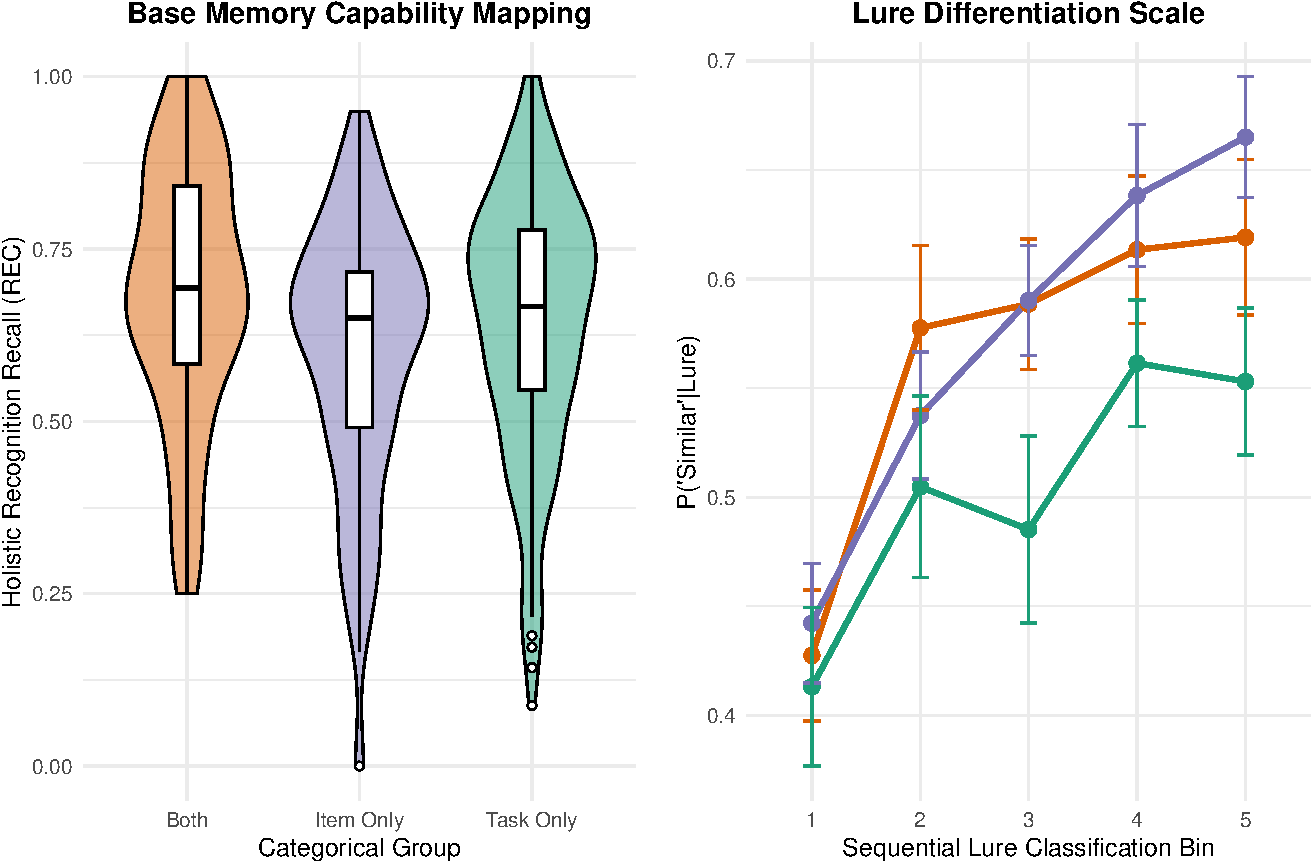
\includegraphics[width=0.6\linewidth]{fig_validations-1}
\caption{\label{fig:validations} Benchmark distributions illustrating data structure. Left: Violin plots of Recognition Memory (REC) across task groups. Right: Line plots showing the relationship between lure similarity (Lure Bin) and the probability of responding “similar” to lure items.}
\end{figure}

The violin plots (left panel) show that overall recognition performance is relatively consistent across groups, with moderate variability and slight skewness typical of behavioural data. No extreme outliers or irregular distributions are observed, indicating that the dataset is suitable for further statistical analysis.

The lure discrimination curves (right panel) display a clear increasing trend across lure bins, where Bin 1 represents highly similar lures (very close to the original “old” items) and Bin 5 represents less similar lures (more distinct from the original items). As the bin number increases, the probability of correctly identifying a lure as “similar” also increases. This pattern is consistent across all groups and aligns with theoretical expectations, as highly similar lures (Bin 1) are more difficult to distinguish from previously seen items, whereas less similar lures (Bin 5) are easier to correctly classify.

Overall, these patterns confirm that the dataset exhibits stable and interpretable structure, providing a reliable foundation for subsequent inferential modelling.

\section{Results: Boundary Disruption Effect (H1)}

To test whether event boundaries disrupt recognition memory, we fitted a linear mixed-effects model with boundary position as a fixed effect and participant as a random intercept, then evaluated the effect using Type III ANOVA and planned contrasts.

\textbf{Hypothesis (H1):} Recognition accuracy remains stable within events (Pre $\approx$ Mid) but drops after a boundary (Post), reflecting a boundary-induced disruption in memory performance.

\begin{table}[H]
\centering
\caption{Type III ANOVA: Main Effect of Boundary Position on REC (LMM, H1).}
\begin{tabular}{lrrrr}
\toprule
Effect & df (num) & df (den) & F & p-value \\
\midrule
Boundary Position & 2 & 318 & 16.13 & \textbf{< .001} \\
\bottomrule
\end{tabular}
\end{table}

A highly significant main effect of boundary position was observed for REC ($F(2, 318) = 16.13$, $p < .001$). Post-boundary accuracy was significantly lower than mid-event accuracy ($t = -4.93$, $p < .001$), confirming a boundary-related disruption in recognition performance.

\begin{table}[H]
\centering
\caption{Planned contrasts for boundary position effect on REC (H1).}
\begin{tabular}{lrrl}
\toprule
Comparison & $t$-value & p-value \\
\midrule
Mid vs Post & $-4.93$ & \textbf{< .001} \\
Pre vs Post & $-3.79$ & \textbf{< .001} \\
Pre vs Mid  & $0.62$  & $.535$ \\
\bottomrule
\end{tabular}
\end{table}

Planned contrasts confirmed that the post-boundary position was significantly lower than both the mid-event ($t = -4.93$, $p < .001$) and pre-boundary ($t = -3.79$, $p < .001$) positions. Pre and mid did not reliably differ ($t = 0.62$, $p = .535$), indicating that the disruption is localised to the moment of contextual transition. Descriptively, mean REC was $M_{\text{pre}} = 0.665$ ($SD = 0.181$), $M_{\text{mid}} = 0.665$ ($SD = 0.187$), and $M_{\text{post}} = 0.594$ ($SD = 0.205$).

\begin{figure}[H]
\centering
\includegraphics[width=0.6\linewidth]{fig_h1_boundary-1}
\caption{\label{fig:rec_gradient} H1 Result: Recognition accuracy by boundary position. Error bars represent ±1 SE.}
\end{figure}

\textbf{Verdict: Supported.} Recognition accuracy is stable within events but drops sharply after the boundary, confirming a boundary-induced disruption in memory performance.

\section{Results: Cognitive Load Effect (H2)}

To examine how cognitive load influences recognition memory, a $3 \times 3$ mixed-effects ANOVA was conducted with Task Group (between-subjects) and Boundary Position (within-subjects) as factors.

\textbf{Hypothesis (H2):} Recognition accuracy is expected to differ across task conditions, with higher cognitive load leading to lower overall performance compared to lower load conditions.

\begin{longtable}[]{@{}lrrrrrl@{}}
\caption{Results of the Type III Mixed ANOVA examining the effects of Task Group and Boundary Position on recognition memory (REC).}\tabularnewline
\toprule
Term & Sum Sq & Mean Sq & Num DF & Den DF & F-value & p-value \\
\midrule
boundary\_position & 0.541 & 0.270 & 2 & 314 & 16.303 & \textbf{< 0.001} \\
group & 0.645 & 0.323 & 2 & 157 & 4.433 & \textbf{0.0134} \\
boundary\_position:group & 0.123 & 0.031 & 4 & 314 & 1.859 & 0.1174 \\
\bottomrule
\end{longtable}

The ANOVA revealed a significant main effect of task group ($F(2, 157) = 4.433$, $p = 0.013$), confirming that recognition accuracy differs across cognitive load conditions. Participants in higher-load task groups demonstrated lower overall recognition performance compared to those in the baseline Item Only condition.

The main effect of boundary position was also significant ($F(2, 314) = 16.303$, $p < .001$), consistent with H1. However, the interaction between group and boundary position was not statistically significant ($F(4, 314) = 1.859$, $p = 0.117$), indicating that while cognitive load affects overall accuracy, it does not differentially amplify the boundary-related decline.

\begin{figure}[H]
\centering
\includegraphics[width=0.6\linewidth]{fig_h2_interaction-1}
\caption{\label{fig:interact} H2 Result: Cognitive Load × Boundary Position interaction. Higher load reduces overall accuracy, but the boundary disruption pattern is similar across groups.}
\end{figure}

As shown in Figure \ref{fig:interact}, the Task Only and Both conditions exhibit consistently lower recognition accuracy compared to the Item Only group. This demonstrates that the cognitive demands imposed by more complex encoding tasks reduce memory performance broadly, supporting the Cognitive Load Effect.

\textbf{Verdict: Supported.} Higher cognitive load significantly reduces overall recognition accuracy.

Since the main effect of Task Group was statistically significant, Bonferroni-corrected post-hoc pairwise comparisons were conducted to identify which specific groups differed in overall recognition accuracy.

\begin{longtable}[]{@{}lcc@{}}
\caption{Bonferroni-corrected post-hoc pairwise comparisons for Task Group main effect on REC (H2).}\tabularnewline
\toprule
Comparison & Mean Difference & p (Bonferroni) \\
\midrule
Item Only vs Task Only & 0.089 & \textbf{0.010} \\
Item Only vs Both Item \& Task & 0.044 & 0.441 \\
Task Only vs Both Item \& Task & $-$0.045 & 0.430 \\
\bottomrule
\end{longtable}

\textbf{Post-hoc Result:} Item Only participants ($M = 0.685$, $SD = 0.147$) significantly outperformed Task Only participants ($M = 0.596$, $SD = 0.174$; $\Delta M = 0.089$, $d = 0.55$, $p_{\text{Bonf}} = 0.010$), representing a medium-sized cognitive load effect. The comparisons between Item Only and Both Item \& Task ($p_{\text{Bonf}} = 0.441$) and between Task Only and Both Item \& Task ($p_{\text{Bonf}} = 0.430$) did not reach statistical significance after correction. This pattern confirms that higher cognitive load leads to lower overall recognition accuracy, with the most pronounced cost observed in the Task Only condition.

\section{Results: Doppelgänger Effect (H3)}

To examine how perceptual similarity influences memory performance, a GLMM with a logistic link was applied to trial-level lure data, with lure similarity (\texttt{lure\_bin}) and task group as fixed effects and participant as a random intercept.

\textbf{Hypothesis (H3):} Highly similar lure items (Bin 1) are expected to be more difficult to distinguish from target items than less similar lures (Bin 5), resulting in lower discrimination accuracy.

\begin{longtable}{lccccc}
\caption{GLMM results showing fixed effects of lure similarity (Lure Bin) on discrimination accuracy.} \\
\toprule
Parameter Term & Estimate & SE & z-score & p-value \\
\midrule
\endfirsthead

\toprule
Parameter Term & Estimate & SE & z-score & p-value \\
\midrule
\endhead

\bottomrule
\endlastfoot

(Intercept) [Item Only] & -0.285 & 0.133 & -2.15 & \textbf{0.031} \\
lure\_bin [Item Only] & 0.196 & 0.036 & 5.41 & \textbf{< 0.001} \\
group (Task Only) & -0.095 & 0.148 & -0.64 & 0.521 \\
group (Both Item \& Task) & -0.155 & 0.173 & -0.89 & 0.372 \\
lure\_bin:task\_only & 0.042 & 0.045 & 0.95 & 0.343 \\
lure\_bin:Both & -0.056 & 0.052 & -1.08 & 0.282 \\

\end{longtable}

\textbf{Result (Supported):} The analysis revealed a strong effect of lure similarity on memory performance ($\beta = 0.196$, $p < 0.001$). Specifically, participants were much more likely to correctly identify a lure as ``similar'' when it was less visually similar to the original item. In contrast, highly similar lures (Bin 1) were frequently mistaken for previously seen items, leading to lower discrimination accuracy.

Importantly, this pattern was consistent across all task groups. There were no significant differences between groups, and no reliable interaction between lure similarity and task condition. This indicates that the effect of similarity on memory errors operates independently of cognitive load.

This pattern is visualized in Figure \ref{fig:lure_fit}, which shows a monotonic increase in accuracy across similarity bins.

\begin{figure}[H]
\centering
\includegraphics[width=0.6\linewidth]{fig_h3_lure-1}
\caption{\label{fig:lure_fit} H3 Result: Lure discrimination by similarity bin. Less similar lures (higher bin numbers) are identified more accurately across all groups.}
\end{figure}

\textbf{Verdict: Supported.} Perceptual similarity is a robust and consistent driver of memory errors, independent of task demands.

\section{Results: Encoding Update Cost (H4)}

To assess the cognitive cost of event model updating during encoding, we examined reaction times across the three boundary-defined positions (Post, Mid, Pre) within each event sequence using a Linear Mixed-Effects Model (LMM) with participant as a random intercept.

\textbf{Hypothesis (H4):} Reaction time is expected to increase immediately following an event boundary, reflecting the cognitive cost of updating the active event model.

\begin{figure}[H]
\centering
\includegraphics[width=0.6\linewidth]{fig_h4_encoding_rt-1}
\caption{\label{fig:enc_rt_gradient} H4 Result: Encoding reaction time by boundary position. RT spikes immediately after boundaries, indicating processing cost of context updating.}
\end{figure}

\begin{table}[H]
\centering
\caption{LMM Results for Encoding Position RT (H4).}
\begin{tabular}{lrrrrl}
\toprule
Position & Estimate (s) & Std.\ Error & t-value & p-value \\
\midrule
Post (Base) & 2.050 & 0.058 & 35.51 & \textbf{< .001} \\
Pre vs Post & $-$0.148 & 0.019 & $-$7.84 & \textbf{< .001} \\
Mid vs Post & $-$0.138 & 0.019 & $-$7.31 & \textbf{< .001} \\
\bottomrule
\end{tabular}
\end{table}

\textbf{Result (Supported):} Encoding reaction time was highest at the post-boundary position, the first item following each event boundary. Both pre-boundary and mid-event positions showed significantly lower RT (Pre vs Post: $t = -7.84$, $p < .001$; Mid vs Post: $t = -7.31$, $p < .001$), confirming that the cognitive cost of updating the active event model is concentrated at the boundary and diminishes as the event representation stabilises. \textbf{Verdict: Supported.}

\section{Discussion and Phenomenological Constraints}
\label{discussion-and-phenomenological-constraints}

The primary objective of Report 2 was to extend the descriptive findings of Report 1 using more rigorous statistical modeling. By applying linear mixed-effects models, mixed ANOVA, and a trial-level GLMM, we aimed to precisely characterize how event boundaries and perceptual similarity influence memory performance in the Mnemonic Similarity Task.

\subsection{Resolution of Targeted Hypotheses}

The combined analyses provide a coherent account of how memory is structured around event boundaries:

\begin{enumerate}
\item
\textbf{Boundary Disruption Effect (H1) — Supported:}
A linear mixed-effects model revealed a significant main effect of boundary position on REC ($F(2, 318) = 16.13$, $p < .001$). Planned contrasts confirmed that post-boundary accuracy was significantly lower than mid-event accuracy ($t = -4.93$, $p < .001$) and pre-boundary accuracy ($t = -3.79$, $p < .001$), while pre and mid did not differ, demonstrating that disruption is localised to the contextual transition.

\item
\textbf{Cognitive Load Effect (H2) — Supported:}
A significant main effect of task group ($F(2, 157) = 4.433$, $p = 0.013$) confirms that higher cognitive load reduces overall recognition accuracy. Participants in more demanding task conditions performed worse than those in the Item Only baseline.

\item
\textbf{Doppelgänger Effect (H3) — Supported:}
A strong and highly significant effect of lure similarity ($\beta = 0.196$, $p < 0.001$) demonstrates that perceptual overlap is a primary driver of memory errors. This effect was consistent across all task groups, indicating that similarity-driven interference operates independently of cognitive load.

\item
\textbf{Encoding Update Cost (H4) — Supported:}
Encoding reaction time was highest at the post-boundary position, with pre-boundary and mid-event positions showing significantly lower RT ($p < .001$ for both). This confirms that the cognitive cost of updating the active event model is concentrated at the boundary.
\end{enumerate}

\subsection{Theoretical Implications}

These findings align closely with Event Segmentation Theory (Zacks et al., 2007), which proposes that perceptual systems partition continuous experience into discrete events. The observed post-boundary decline supports the idea that memory updating at event transitions temporarily disrupts encoding processes.

Crucially, the results indicate that this disruption is:
\begin{itemize}
\item \textbf{Position-specific} (H1): accuracy drops at the boundary itself, not gradually,
\item \textbf{Load-sensitive at a global level} (H2): cognitive demand lowers overall performance,
\item \textbf{Complemented by perceptual interference} (H3): driven by stimulus similarity,
\item \textbf{Manifest during encoding} (H4): RT peaks at the post-boundary position, reflecting active event model updating.
\end{itemize}

This suggests that boundary-related memory disruption and similarity-based interference operate as \textbf{independent mechanisms} shaping memory performance.

\subsection{Constraints and Future Directions}

Several limitations should be noted. First, the use of discrete boundary positions (Pre, Mid, Post) simplifies what is likely a continuous encoding process. Second, the reliance on binary response models (correct vs incorrect) may obscure more nuanced memory dynamics. Finally, the absence of neural measures limits direct interpretation of underlying cognitive mechanisms.

Future work could extend these findings by incorporating continuous-time modeling, neuroimaging data, or adaptive boundary manipulations to better isolate the mechanisms of boundary-driven memory disruption.

\subsection{Overall Hypothesis Summary}

\begin{longtable}[]{@{}
  >{\raggedright\arraybackslash}p{(\linewidth - 4\tabcolsep) * \real{0.25}}
  >{\raggedright\arraybackslash}p{(\linewidth - 4\tabcolsep) * \real{0.60}}
  >{\raggedright\arraybackslash}p{(\linewidth - 4\tabcolsep) * \real{0.15}}@{}}
\caption{\label{tab:hypo} Summary of hypothesis outcomes.}\tabularnewline
\toprule
Hypothesis & Description & Status \\
\midrule
Boundary Disruption Effect (H1) & Recognition accuracy stable within events but drops sharply at post-boundary & Supported \\
Cognitive Load Effect (H2) & Higher cognitive load leads to lower overall recognition accuracy & Supported \\
Doppelgänger Effect (H3) & Highly similar lures are harder to distinguish, lowering discrimination accuracy & Supported \\
Encoding Update Cost (H4) & RT is highest at the post-boundary position during encoding, reflecting event model updating cost & Supported \\
\bottomrule
\end{longtable}

\section{Conclusion}\label{conclusion}

This sequence of statistical analyses extends the descriptive findings from Report 1 by providing a more precise and statistically grounded understanding of how event boundaries and perceptual similarity influence memory performance in the Mnemonic Similarity Task.

The \textbf{Boundary Disruption Effect (H1)} was supported. A linear mixed-effects model with Type III ANOVA confirmed a significant main effect of boundary position on recognition accuracy ($F(2, 318) = 16.13$, $p < .001$). Planned contrasts showed that post-boundary accuracy was significantly lower than mid-event accuracy ($t = -4.93$, $p < .001$) and pre-boundary accuracy ($t = -3.79$, $p < .001$), while pre and mid did not differ. This confirms that memory disruption is localised to the moment of contextual transition.

The \textbf{Cognitive Load Effect (H2)} was supported. A significant main effect of task group ($F(2, 157) = 4.433$, $p = 0.013$) confirmed that participants in higher-load conditions exhibited lower overall recognition accuracy. Post-hoc comparisons showed that the Item Only vs Task Only contrast reached significance ($\Delta M = 0.089$, $d = 0.55$, $p_{\text{Bonf}} = 0.010$), with the Both Item \& Task group showing intermediate performance. The interaction between boundary position and cognitive load was not significant ($p = 0.117$), indicating that while cognitive load reduces memory globally, the boundary disruption pattern is consistent across all groups.

The \textbf{Doppelgänger Effect (H3)} revealed that perceptual similarity is a robust driver of memory errors ($\beta = 0.196$, $p < 0.001$). Highly similar lures were frequently mistaken for previously seen items, while less similar lures were correctly identified more often. This effect was consistent across all task groups, operating independently of cognitive load.

The \textbf{Encoding Update Cost (H4)} provided converging evidence from the encoding phase. Reaction time was highest at the post-boundary position and decreased significantly at pre-boundary and mid-event positions (both $p < .001$), confirming that the cognitive cost of updating the active event model is concentrated at the boundary.

Taken together, all four hypotheses were supported. These findings indicate that memory performance is shaped by three primary mechanisms: (1) a position-specific disruption at event boundaries visible in both encoding RT and retrieval accuracy, (2) a global reduction in performance under higher cognitive load (most pronounced for the Task Only group), and (3) a strong influence of perceptual similarity on discrimination accuracy. Importantly, these mechanisms appear to operate largely independently, highlighting the distinct roles of event segmentation, cognitive demand, and stimulus similarity in structuring memory.


\section*{Author Contributions}\label{author-contributions}
\addcontentsline{toc}{section}{Author Contributions}

All three authors contributed equally to this project. Each member was responsible for at least one hypothesis, the corresponding statistical implementation in R, and associated written sections.

\begin{itemize}

  \item \textbf{Srushti Pekamwar} — \textit{Hypotheses: H1 (Boundary Disruption Effect) and H4 (Encoding Update Cost).}
  Responsible for data cleaning, merging of raw task and test files, and construction of trial-level encoding and retrieval datasets. Implemented the LMM and Type III ANOVA for H1 (\texttt{lmer(REC \textasciitilde{} boundary\_position + (1|participant))}) with planned contrasts, and the LMM for H4 (\texttt{lmer(encoding\_RT \textasciitilde{} boundary\_pos + (1|participant))}). Generated the positional REC gradient figure and the encoding RT figure. Drafted the H1 and H4 Results subsections and the Discussion.

  \item \textbf{Anurag Kaushal} — \textit{Hypotheses: H2 (Cognitive Load Effect).}
  Responsible for participant-level metric computation (REC, LDI) and data validation diagnostics. Implemented the $3 \times 3$ mixed-effects ANOVA (\texttt{lmer(REC \textasciitilde{} boundary\_position * group + (1|participant))}) for H2, including the group main effect, boundary$\times$group interaction test, and interaction plot. Also contributed to the GLMM pipeline setup and random-effects forest plot. Drafted the Methods section and the Data Validation subsection.

  \item \textbf{Param Modi} — \textit{Hypothesis: H3 (Doppelg\"{a}nger Effect).}
  Responsible for literature review and theoretical framing of Event Segmentation Theory. Implemented the binomial GLMM for H3 (\texttt{glmer(accuracy \textasciitilde{} lure\_bin * group + (1|participant), family = binomial)}) and generated the lure similarity interaction and facet plots. Constructed the hypothesis summary table and ROC/heatmap supplementary figures. Drafted the Introduction, H3 Results subsection, Conclusion, and coordinated the final report compilation and poster preparation.

\end{itemize}

\section*{References and Citations}\label{references-and-citations}
\addcontentsline{toc}{section}{References and Citations}

Morse, S. J., Karagoz, A. B., \& Reagh, Z. M. (2023). Event boundaries
influence item-level recognition memory.

Stark, S. M., Kirwan, C. B., \& Stark, C. E. L. (2019). Mnemonic
similarity task. \emph{Trends in Cognitive Sciences}.

Yassa, M. A., \& Stark, C. E. L. (2011). Pattern separation in the
hippocampus. \emph{Trends in Cognitive Sciences}.

Swallow, K. M., Zacks, J. M., \& Abrams, R. A. (2009). Event boundaries
and memory encoding. \emph{Journal of Experimental Psychology:
General}.

Zacks, J. M., Speer, N. K., Swallow, K. M., et al. (2007). Event
perception. \emph{Psychological Bulletin}.

\begin{center}\rule{0.5\linewidth}{0.5pt}\end{center}

\end{document}
